\section{Results}\label{results}
In this section we will describe our results both locally against our self and
against two other groups in a tournament setting.

\subsection{Local}\label{results:local}
One of the first things we wanted to know when we had created our minimax 
implementation is when we should switch. As the first few positions have very
little bearing on the rest of the game, we can play a few moves as a novice
before switching to the minimax algorithm. To test when this switch should
occur we played our minimax algorithm against it self in a number of scenarios
to see when we should switch. 

\begin{figure}[h]
	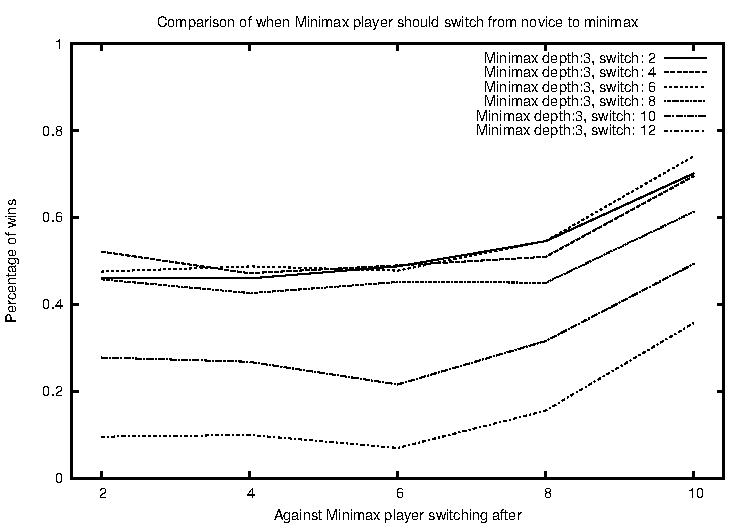
\includegraphics{graphs/switch.pdf}
	\caption[Minimax switch graph]{Graph describing our minimax switch results}
	\label{fig:minimax switch}
\end{figure}

We ran the code in listing \ref{lst:switch code} and got the results you can see in figure
\ref{fig:minimax switch}. From this we can see that switching on 2, 4 and 6 is 
really not any different.
The small difference we can see is just random variance because of the single
run we have tested. When we get down to switching after 8 pieces has been placed
there is some difference and we start to see a drop in efficiency.

Below are the results that we got from running our implementation against it self.
Each result has a corresponding listing in appendix \ref{run configuration} where
we have added the commands to duplicate our results.

\begin{table}[btp]
	\centering
	\begin{tabular}{| l | l | l | l |}
		\hline
		Player type & Wins(\%) & Loses(\%) & Ties(\%)\\
		\hline
		Random & 9 (1\%) & 488 (97\%) & 3 (0.6\%)\\
		Novice & 488 (97\%) & 9 (1\%) & 3 (0.6\%)\\
		\hline
	\end{tabular}
	\caption{Table showing Random compared to Novice player. See listing
	\ref{lst:novice vs random} for command}
	\label{table:random vs novice}
\end{table}
\begin{table}[btp]
	\centering
	\begin{tabular}{| l | l | l | l |}
		\hline
		Player type & Wins(\%) & Loses(\%) & Ties(\%)\\
		\hline
		Minimax 3 6 & 472 (94\%) & 20 (4\%) & 8 (1.6\%)\\
		Novice & 20 (4\%) & 472 (94\%) & 8 (1.6\%)\\
		\hline
	\end{tabular}
	\caption{Table showing Novice compared to Minimax player using depth 3
	and switching after 6 pieces placed. See listing \ref{lst:novice vs minimax}
for command}
	\label{table:minimax vs novice}
\end{table}

\begin{table}[btp]
	\centering
	\begin{tabular}{| l | l | l | l |}
		\hline
		Player type & Wins(\%) & Loses(\%) & Ties(\%)\\
		\hline
		Minimax 3 6 & 47 (9\%) & 207 (41\%) & 246 (49\%)\\
		Minimax 4 6 & 207 (41\%) & 47 (9\%) & 246 (49\%)\\
		\hline
	\end{tabular}
	\caption{Table showing Minimax 3 6 compared to Minimax 4 6. See listing
	\ref{lst:minimax3 vs minimax4} for command}
	\label{table:minimax3 vs minimax 4}
\end{table}

From this results we can see that our Random player is truly living up to its
name and losing almost all of the time. Our Novice player can hold its ground
against the Random player, but will lose a few times most likely attributed to
it not detecting guaranteed losing situations a head of time. As one can see our
Minimax player does quite well and even better when allowed to search further
down the tree. It will lose a couple of times against Novice, but this is attributed
to the late switching and some states which our heuristics can't detect(Please see
section \ref{future work} for some extensions which could detect more of these).

\subsection{Tournament}\label{results:tournament}
The tournament went quite well for us and we did quite good. One of the strengths
we had compared to the others were the Python/C implementation which made quite
a drastic impact on the time we used in the tournament(as can be seen in table 
\ref{table:tournament time}). In table \ref{table:tournament result} we have 
our raw statistics from the tournament. The tournament was ran for
eight(8) hours and each player got a total of 822 games played.

\begin{table}[btp]
	\centering
	\begin{tabular}{| l | l | l | l |}
		\hline
		Player name & Wins(\%) & Loses(\%) & Ties(\%)\\
		\hline
		Abraham & 356 (43\%) & 238 (29\%) & 228 (28\%)\\
		Mikkel & 196 (24\%) & 444 (54\%) & 182 (22\%)\\
		Trond \& Jørgen & 366 (45\%) & 236 (28\%) & 220 (27\%)\\
		\hline
	\end{tabular}
	\caption{The tournament result}
	\label{table:tournament result}
\end{table}

\begin{table}[btp]
	\centering
	\begin{tabular}{| l | l |}
		\hline
		Player name & Time used in seconds\\
		\hline
		Abraham & 7401 (26\%) \\
		Mikkel & 18250 (63\%) \\
		Trond \& Jørgen & 3352 (11\%) \\
		\hline
	\end{tabular}
	\caption{Time spent in the tournament calculating}
	\label{table:tournament time}
\end{table}
